\chapter{Background Information}\label{ch02}

\section{Background Information}

\subsection{Le Chateliers principle}

Le Chateliers principle is essential for understanding equilibrium equations, and his principle states that a reaction at equilibrium will continue to stay in equilibrium unless an external force causes disturbance, where the system will try to create a new equilibrium state. Le Chatelier had first come up with his principle in 1884 and had later finalised it in 1933 (Lower, 2024).

\begin{center}
    \textit{“If a dynamic equilibrium is disturbed by changing the conditions, the position of equilibrium shifts to counteract the change.” } (Le Chatelier, 1884)
\end{center}

This essentially means that if any factor that affects an equilibrium is altered, the system will adjust to minimise the impact of that change, eventually establishing a new equilibrium.
 The conditions that can cause an equilibrium shift in a system are concentration, temperature, pressure (gas reactions), catalyst’s, and volume changes in a gas system. \\

Le Chatelier states that when the concentration of a reaction is altered, the system will work to return the system back to equilibrium	.
So when a reactant is increased, the forward reaction will be lowered and the equilibrium will be shifted to the right, favouring the reverse reaction. In the opposite reaction, where the product is increased, the reverse reaction will be lowered, shifting the equilibrium to the left, favouring the forward reaction (Davis, Disney, and Smith, 2018). \\

A simplified way to say this is to consider if you were in your room, consider the following: 

\begin{figure}[htp]
    \centering
    \[
        Clean \ Room \rightleftharpoons Messy \ Room
    \]
    \caption{}
    \label{fig:enter-label}
\end{figure}

If the room is clean, you might leave your socks and clothes on the floor; in this way, you increase the concentration of messiness in your room, which in turn makes the reverse reaction more favourable where you clean your room, but once your room is clean, the concentration of messiness is lower than the concentration of cleanliness; in turn, you mess up your room again, leading to an equilibrium. (Ihde, 1989). \\

Pressure and temperature also play important roles in the equilibrium of a system. Le Chatelier states that in gaseous reactions, when the pressure is increased, the equilibrium will shift to the side with fewer moles, and when the pressure is decreased, the reverse will happen, where the reaction with more moles is favoured (Davis, Disney, and Smith, 2018). \\

The production of methanol, which includes combining carbon monoxide gas and hydrogen gas, is typically performed under a high pressure (100 atm); this allows for a maximum yield of methanol, making it more suitable for commercial applications. 

\begin{figure}[htp]
    \centering
    \[
       CO (g) + 2H_{2} (g) \rightleftharpoons CH_{3}OH(g) \\
    	\Delta H = -90.7 kJ/mol
    \]
    \caption{}
    \label{fig:enter-label}
\end{figure}

In this reaction, there is a 3:1 ratio of gas molecules, where there is one carbon monoxide molecule and two hydrogen moles to 1 methanol molecule on the right. In this system, if the volume were to decrease by two, the pressure of the system would increase by two in turn. The increased pressure of the system would make it so there are more molecules colliding, favouring the forward reaction with fewer moles until equilibrium is reached. \\

For a system at equilibrium, when temperature is altered, the system would work to go back into equilibrium. Le Chateliers Principle states that when the temperature is increased within a system, the reaction that is endothermic (absorbs heat) will be favoured until the system reaches a state of equilibrium again; when the temperature is decreased within a system, the exothermic (releasing heat) reaction will be favoured until equilibrium is reached again. \\

Consider the following reaction below: 

\begin{figure}[htp]
    \centering
    
    % https://q.uiver.app/#q=WzAsOSxbMCwwLCJOaXRyb2dlbiJdLFswLDEsIlxcYnVsbGV0Il0sWzAsMiwiSHlkcm9nZW4gXFxcXCBGcm9tIFxcIE5hdHVhbCBcXCBHYXMiXSxbMSwwLCJOaXRyb2dlbiBcXCBBbmQgXFwgSHlkcm9nZW4gXFxcXCAxOjMgXFwgUmF0aW8iXSxbMiwxLCJJcm9uIFxcIENhdGFseXN0IFxcXFwgNDAwXm8gQyBcXCAyMDBhdG0iXSxbMiwyLCJHYXMgXFwgY29vbGVkIFxcIHRvIFxcIGZvcm0gXFxcXCBsaXF1aWQgXFwgYW1tb25pYSJdLFsxLDEsIlxcYnVsbGV0Il0sWzIsMywiXFxidWxsZXQiXSxbMSwzLCJcXGJ1bGxldCJdLFswLDFdLFsyLDFdLFsxLDRdLFs0LDVdLFs1LDddLFs3LDgsIlVudXNlZCBcXCBHYXNzZXMgXFwgUmVjeWNsZWQiXSxbOCw2XV0=
    \begin{tikzcd}
	Nitrogen & \begin{array}{c} Nitrogen \ And \ Hydrogen \\ 1:3 \ Ratio \end{array} \\
	\bullet & \bullet & \begin{array}{c} Iron \ Catalyst \\ 400^o C \ 200atm \end{array} \\
	\begin{array}{c} Hydrogen \\ From \ Natual \ Gas \end{array} && \begin{array}{c} Gas \ cooled \ to \ form \\ liquid \ ammonia \end{array} \\
	& \bullet & \bullet
	\arrow[from=1-1, to=2-1]
	\arrow[from=2-1, to=2-3]
	\arrow[from=2-3, to=3-3]
	\arrow[from=3-1, to=2-1]
	\arrow[from=3-3, to=4-3]
	\arrow[from=4-2, to=2-2]
	\arrow["{Unused \ Gasses \ Recycled}", from=4-3, to=4-2]
\end{tikzcd}
    \caption{Production of Ammonia}
    \label{fig:enter-label}
\end{figure}

\newpage

In this reaction, the forward reaction is exothermic and had a heat enthaply of \begin{math}\Delta H \end{math}. In this reaction, an iron catalyst is combined with potassium hydroxide to increase the efficiency of the reaction; additionally, the pressure that most manufacturing plants use is 200 atm or over. Using Le Chatelier’s Principle, increasing the pressure of a system will favour the reaction that produces the lowest amount of molecules; in the Habes process, the left-hand side of the process has 4 molecules and the right-hand side has 2 molecules. This is used to get the maximum amount of ammonia in the manufacturing process (Clark, 2023)

\subsection{Collision Theory}
Collision theory was first theorised by two chemists, Max Trautz in 1916 and William Lewis in 1918 (Fleming, 2021). Collision theory states that all reactions occur due to particles colliding with each other; this explains why different reactions occur at different rates, as more collisions would lead to a faster reaction (Byjus, 2011). \\
It is stated that for a reaction to occur, it must first collide with another particle, have enough energy to start the reaction (activation energy), and have the proper orientation (Lawson and Lower, 2023).
The most common equation used to calculate the rate of a reaction according to equilibrium theory is: 
\begin{math} Rate = Z_{ab}F \end{math}

In this equation, \begin{math} Rate = Z_{ab}F \end{math} represents the frequency of collisions between molecules A and B, and F is the amount of collisions that will lead to a successful reaction occurring.
Increasing the number of collisions in a system typically increases the rate of reaction. Factors that can influence this are: \\

\subsubsection{Concentration and Volume}
Having a higher concentration of particles within system will lead to more collisions per second. \\

\begin{figure}
    \centering
    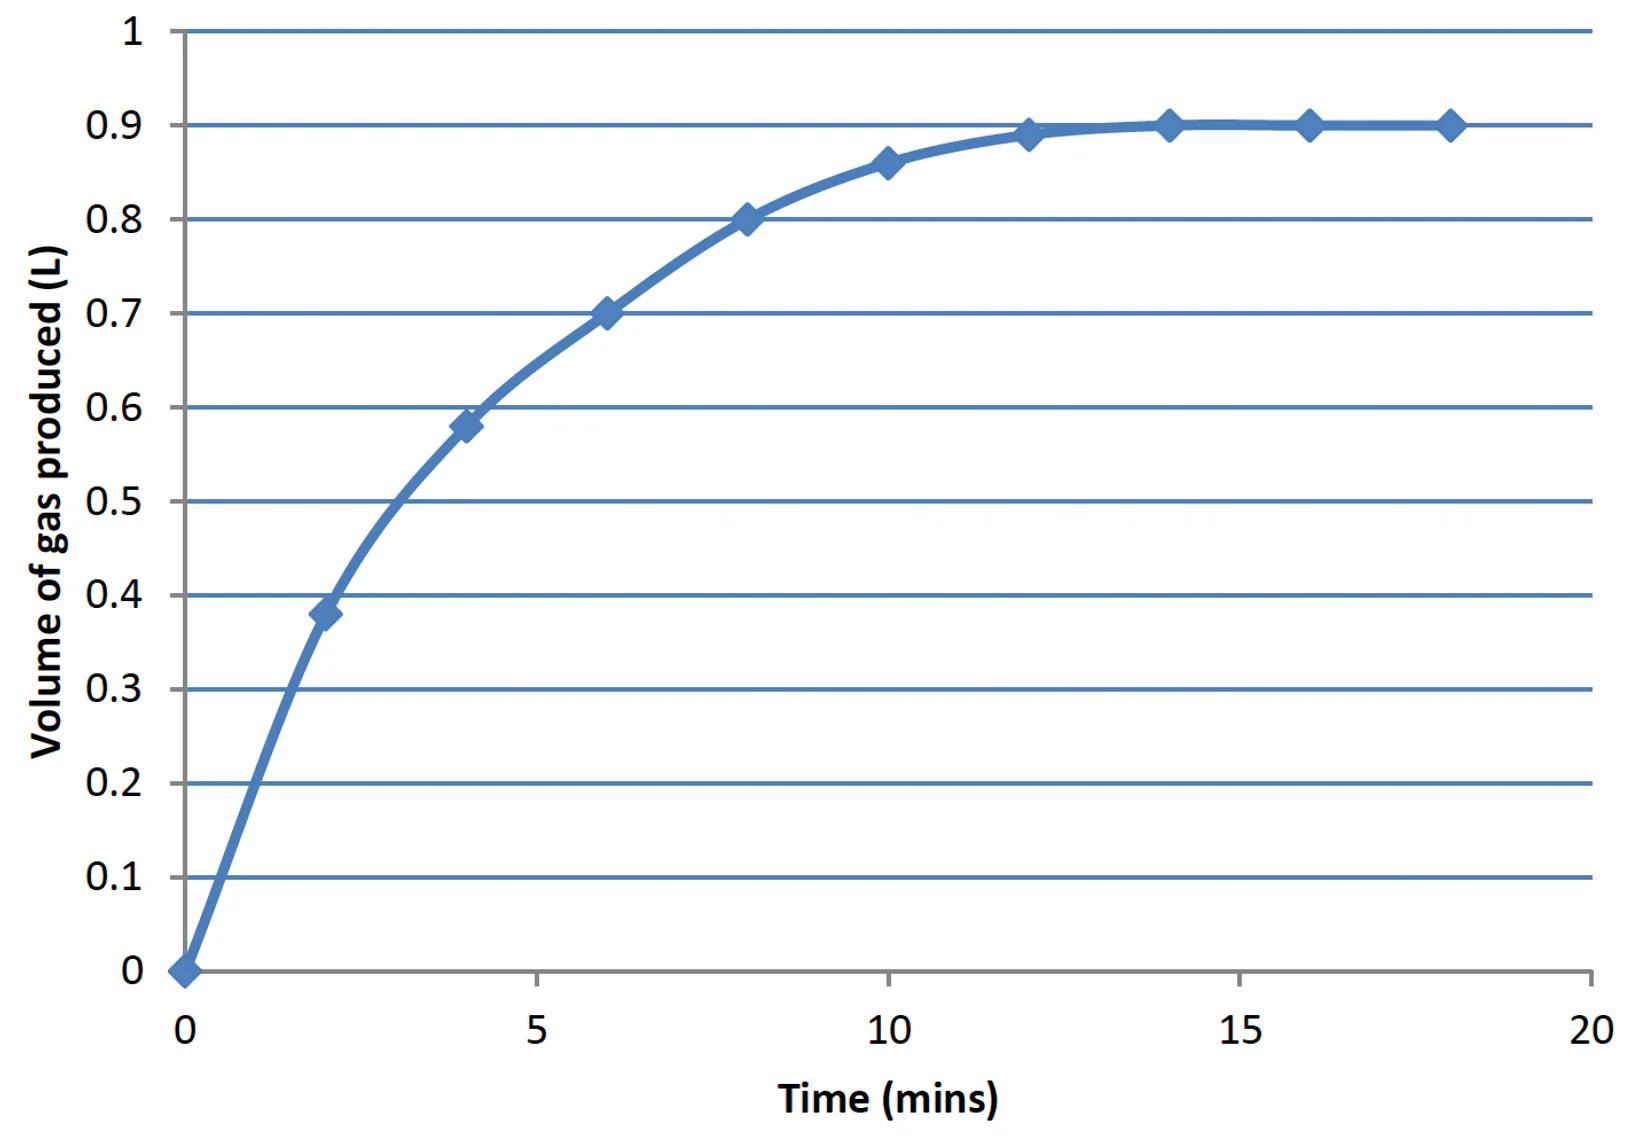
\includegraphics[width=1\linewidth]{assets/1.jpg}
    \caption{As time goes on and more gas is produced, pressure will increase.}
    \label{fig:enter-label}
\end{figure}

\newpage

As a reaction takes place, the concentration of the reaction will be lowered, leading to fewer reactions, and thus the reaction rate decreases over time, until reaching zero when the limiting reagent is completely used up. \\
Pressure/Volume also increases the rate of reaction in gaseous reactions due to their being less room for the particles to go, so they collide with each other more often in a smaller space (Science Ready, 2019).

\subsubsection{Temperature}
In a system, a higher temperature would lead to a higher kinetic energy of particles; this makes the particles move faster, which leads to them colliding more frequently with higher energy, increasing the reaction rate (Science Ready, 2019).
Kinetic energy energy is given as

\begin{figure}[htp]
    \centering
    \[
         K = 1/2 mv^2 \\
        Where \\
        m = particle mass \\
        v  = speed
    \]
    \caption{}
    \label{fig:enter-label}
\end{figure}

\begin{figure}[htp]
    \centering
    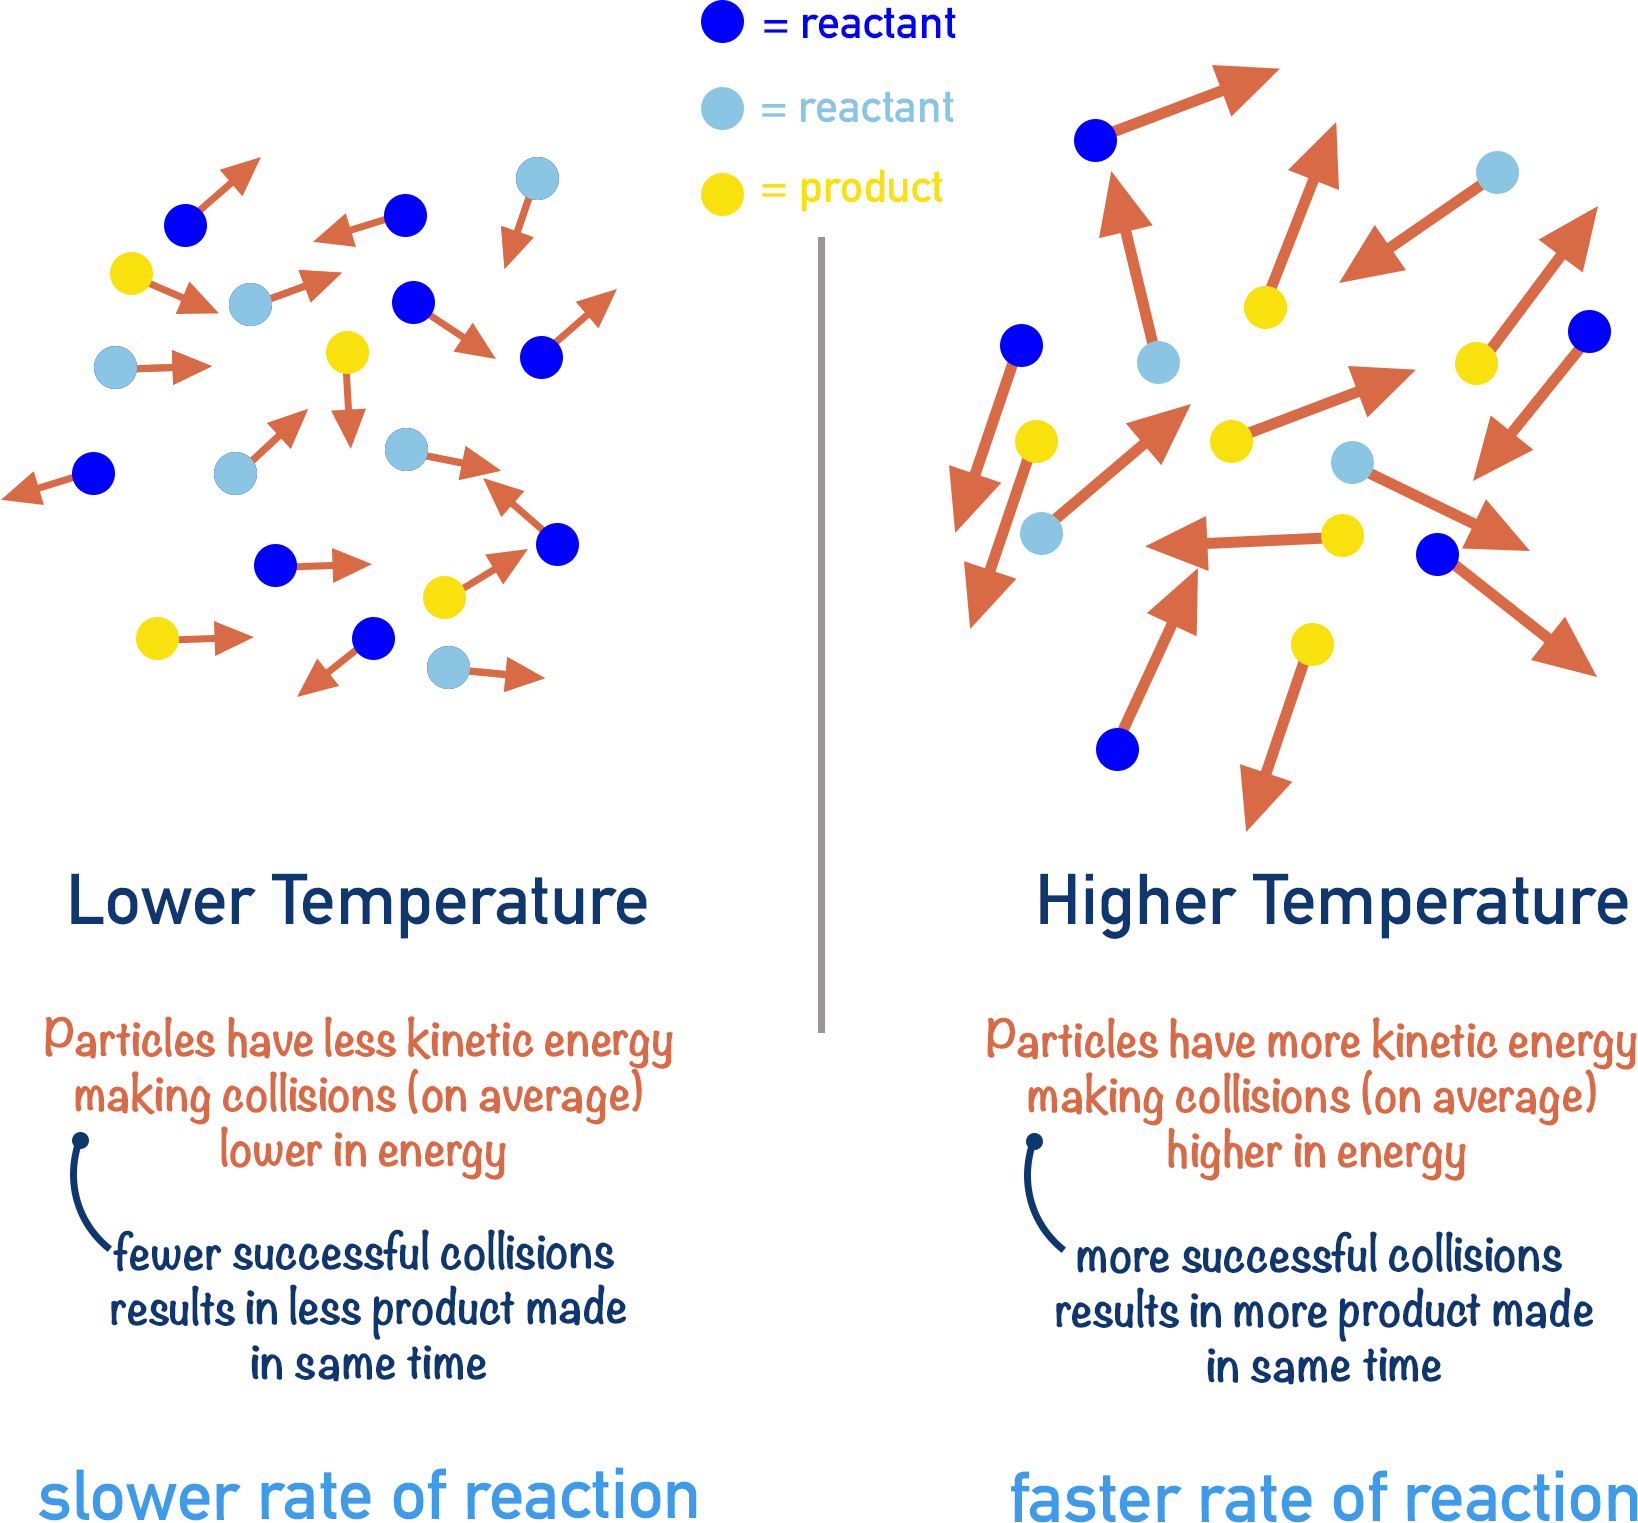
\includegraphics[width=0.5\linewidth]{assets/8.png}
    \caption{Affect of temperature in collision theory}
    \label{fig:enter-label}
\end{figure}

\subsubsection{Surface Area}
Increasing the surface area in a reaction by crushing the reactants into a power, such as iron powder in a thermite reaction, can increase the rate of reaction by allowing more iron to be melted by the reaction. \\
Think of it as having a cup of water. In a cup, the water is only exposed to the top of the cup, and it may be quite small; however, when you spill it across a counter top, the water gets more area in which it can interact and collide with other particles. So which would react faster? putting a block of iron outside to rust or putting iron shavings outside to rust. It would obviously be the iron shavings due to them having a greater surface area when compared to the iron block (Dillon, 2024).



\subsubsection{Catalysts}

A catalyst is a product that can be used within a chemical reaction that lowers the activation energy, thus speeding up the rate of reaction within a system. It is important to note that a catalyst is not used up in a reaction, nor does it move the position of equilibrium; it is only there to fasten the reaction to a state of equilibrium; after reaching equilibrium, the catalyst will no longer affect the reaction. \\

In many industrial processes, the use of catalysts is widespread as they help reduce the time or energy required to start a chemical reaction. 
An example of this can be seen in Figure 2.3 in the production of ammonia a iron catalyst is used to lower the energy required to convert nitrogen and hydrogen gas into liquid ammonia.

\newpage

\subsubsection{Example}
Consider the following dynamic equilibrium equation: 

\begin{figure}[htp]
    \centering
    \[
        2NO_{2}(g) \rightleftharpoons N_{2}O_{4}(g) \\

	Initial Concentrations \\
	2NO_{2}(g) : 0 mol L^-1	\\ N_{2}O_{4}(g) : 0.5 mol L^-1
    \]
    \caption{}
    \label{fig:enter-label}
\end{figure}

In this reaction, \begin{math}N_{2}O_{4}(g)\end{math} will decompose in its reverse reaction to form \begin{math}NO_{2}(g)\end{math} molecules. Initially the concentration of \begin{math}N_{2}O_{4}(g)\end{math} is high, and this means there are lots of collisions occurring. As time goes on, the forward reaction slows down as more \begin{math}N_{2}O_{4}(g)\end{math} molecules are formed, eventually reaching a dynamic equilibrium where both forward and reverse rates are occurring at the same rate (Scienceready, 2019).

\begin{figure}
    \centering
    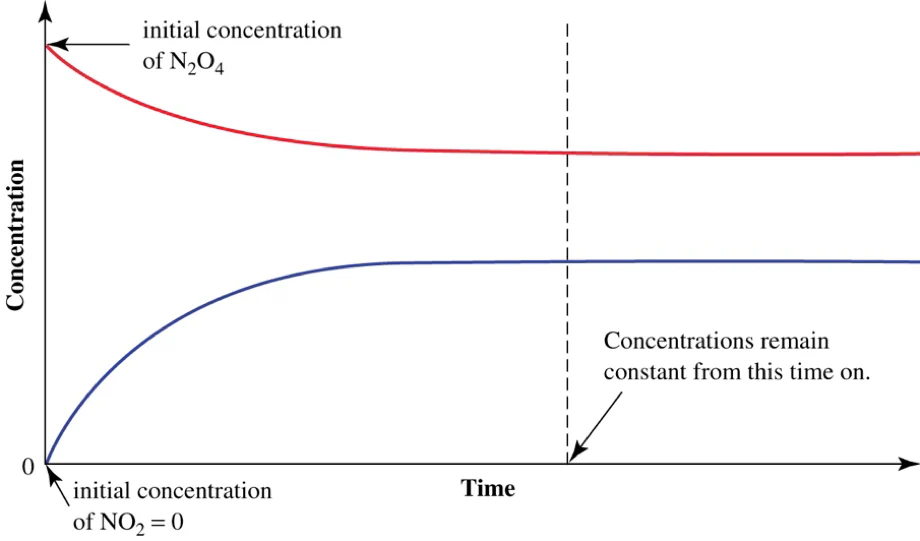
\includegraphics[width=1\linewidth]{assets/2.jpg}
    \caption{Concentration of \begin{math}N_{2}O_{4}\end{math} and \begin{math} NO_{2}\end{math} reaching equilibrium as forward and reverse reactions occur at the same rate.}
    \label{fig:enter-label}
\end{figure}
\newpage

\subsection{Activation Energy and Reaction Rate}
The law of activation energy, otherwise known as the Arrhenius law, states the minimum kinetic or potential energy needed to stretch, bend, or break bonds to start a chemical reaction. This minimum energy is known as the activation energy and is commonly expressed as \begin{math}E_{a}\end{math} (Bui et al., 2022). \newpage

\begin{figure}
    \centering
    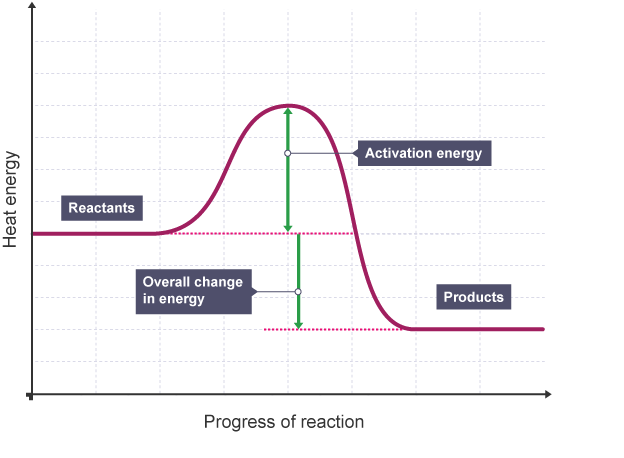
\includegraphics[width=0.5\linewidth]{assets/3.png}
    \caption{Activation energy graph (BBC Bitesize, 2021)}
    \label{fig:enter-label}
\end{figure}

The activation energy (\begin{math}E_{a}\end{math}) is also known as the transition state and is the point at which the most energy is in the system. So if the molecules reacting have an energy higher than the transition state energy, the reaction will continue; this means if a reaction has a very high activation energy, more energy is needed to start the reaction (Bui et al., 2022).

\section{Equilibrium constant}
The equilibrium constant is usually denoted as K, and it provides information about the relationship of products and reactants in a chemical reaction at equilibrium. Equilibrium constant of concentration is denoted as \begin{math}K_{c}\end{math} and is the ratio of the concentration of products to the concentration of the reactants, each raised to their respective stoichiometric coefficients. \\

For a generic reverse reaction equation: 

\begin{figure}[htp]
    \centering
    \[
        aA + bB \rightleftharpoons cC + dD
    \]
    \caption{}
    \label{fig:enter-label}
\end{figure}

The equilibrium constant would be calculated as:

\begin{figure}[htp]
    \centering
    \[
        K_{eq} = \frac{[C]^c \ [D]^d}{[A]^a \ [B]^b} \\ 
        Where: \\
        K > 1 : Products are favoured at equilibrium. \\
        K < 1 : Reactants are favoured at equilibrium. \\
	    K = 1 : Both reactants and products are found at roughly the same amounts.
    \]
    \label{fig:enter-label}
\end{figure}
\newpage

However, in a reaction that included gases, the equilibrium constant would be calculated using \begin{math}K_{p}\end{math}, as P is the partial pressure of the system.

\begin{figure}[htp]
    \centering
    \[
        K_{p} = \frac{[P_{C}]^c \ [P_{D}]^d}{[P_{A}]^a \ [P_{B}]^b}
    \]
    \caption{}
    \label{fig:enter-label}
\end{figure}

So in an equilibrium system, the equilibrium constant can be used to see if the forward or reverse reactions are more favourable or if the system has roughly equal parts reactants and products.










